% =====================================================================
%  Keep the Referent: Anchor-Preserving Token Compression for
%  Privacy-Aware Inference on IoT Logs
%
%  LaTeX V1 —— 分章节草稿
%
%  编译方式（Overleaf 或本地 TeX Live）：
%     pdflatex main
%     bibtex   main
%     pdflatex main
%     pdflatex main
%
%  章节文件位于 sections/，表格位于 tables/，图位于 figures/。
%  文中形如 [待填：...] 的方括号是本轮尚未落定的证据或著录信息，
%  投稿前必须逐条消除。
% =====================================================================

\documentclass[10pt,twocolumn]{article}

\usepackage[T1]{fontenc}
\usepackage[utf8]{inputenc}
\usepackage{times}
\usepackage{microtype}
\usepackage{amsmath,amssymb}
\usepackage{graphicx}
\usepackage{booktabs}
\usepackage{multirow}
\usepackage{threeparttable}
\usepackage[numbers,sort&compress]{natbib}
\usepackage{xcolor}
\usepackage{url}
\usepackage[hidelinks]{hyperref}
\usepackage{caption}
\usepackage{algorithm}
\usepackage{algpseudocode}
\usepackage{balance}

\captionsetup{font=small,labelfont=bf}
\setlength{\textfloatsep}{9pt plus 2pt minus 2pt}
\setlength{\floatsep}{8pt plus 2pt minus 2pt}
\setlength{\intextsep}{8pt plus 2pt minus 2pt}

% 双栏全宽浮标的放置余量
\renewcommand{\dbltopfraction}{0.92}
\renewcommand{\dblfloatpagefraction}{0.72}
\renewcommand{\topfraction}{0.90}
\renewcommand{\floatpagefraction}{0.70}
\renewcommand{\textfraction}{0.06}
\setcounter{dbltopnumber}{3}
\setcounter{topnumber}{3}
\setcounter{totalnumber}{5}

% 指标方向约定：正文与表头统一用 ↑ 表示越高越好、↓ 表示越低越好
\newcommand{\msr}[1]{\textsc{#1}}
\newcommand{\arm}[1]{\texttt{#1}}

\begin{document}

\title{\bf Keeping the Referent in the DARK: Anchor-Preserving\\ Token Compression for Privacy-Aware Inference on IoT Logs}

\author{%
\begin{tabular}{cc}
Yukun Wen & Shijie Zeng \\[1pt]
{\small\texttt{100069961@ku.ac.ae}} & {\small\texttt{100065732@ku.ac.ae}} \\[7pt]
\multicolumn{2}{c}{\small Department of Computer Science, Khalifa University, Abu Dhabi, United Arab Emirates}
\end{tabular}}
\date{}
\maketitle

\begin{abstract}
IoT device logs are long, identifier-dense, and routinely copied into language-model
prompts. A question about an account names exactly the value that must not reach the model,
so the queried entity is also the entity under protection. Redaction removes the value and,
with it, the handle the reader needs; compression keeps the handle but drops the record that
carries the answer. We show that the two goals need not be traded against each other. In
these logs the record that answers the question and the record that stores the protected
value are the same block, so \textsc{DARK} keeps that block and aliases the values inside it.

The rule is training-free: it labels each unit on sensitivity and relevance, applies
one of four operations---delete, alias, refill, keep---and writes the same alias map
into the question. Relevance is read from the question alone, so the compressor never
consults the reference answer.

On $2{,}728$ cases at a $50\%$ budget \textsc{DARK} reaches F1 $0.4937$, level with the
strongest query-aware compressor ($0.4831$; difference not significant) while leaving $0\%$
of protected values recoverable against that method's $98.1\%$, and exceeds the only leak-free
baseline by $0.3226$ points. On a 112-case set, keeping $48.6\%$ of the tokens is
statistically indistinguishable from aliasing the full context without compression ($0.6366$
vs.\ $0.6475$). Removing the alias step costs $0.3273$ F1 where the anchor is itself a
protected value and $0.0013$ where the question names no entity, so the rule acts where designed
and is inert elsewhere. The ordering holds at every budget from $10\%$ to $75\%$,
across a second reader and two paraphrases.
\end{abstract}


\section{Introduction}
\label{sec:intro}

Operational logs from consumer IoT deployments record what each device did, when, and for
which account. They are long (an excerpt in our benchmark reaches $19{,}838$ tokens),
repetitive, and full of identifiers: account handles, device serials, contact fields. They
are also a natural substrate for question answering. An operator asks which device is
associated with a given account and expects a short answer.

The property that makes such a question answerable is also what makes it unsafe to send
verbatim. The question names an entity, and that entity is itself a protected value.
Redacting it before inference is the standard remedy, and it destroys the task: once the
account handle is gone, the model cannot tell which of two hundred similar records the
question refers to. Compressing the context is the other standard remedy, and it destroys
the task for a different reason. Under a redundancy-ordered rule the record carrying the
answer survives compression in $47.5\%$ of cases on our benchmark, and in only $37.2\%$ of
needle cases, where the answer value repeats across distractor records and the score gives it
no priority. Both remedies treat protecting the value and keeping the reference as competing
goals to be balanced.

\begin{figure*}[t]
\centering
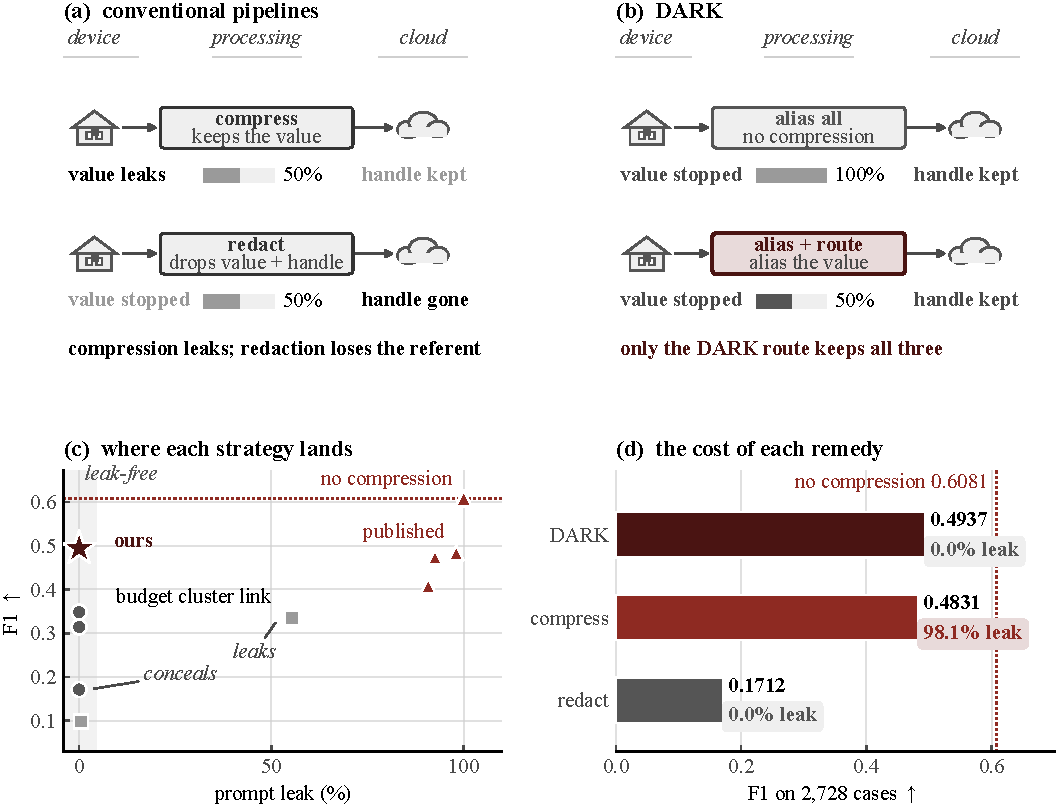
\includegraphics[width=\textwidth]{figures/fig0_teaser.pdf}
\caption{The conflict, and where each strategy lands on it. (a) A question names an account,
and the record that answers it also stores that account as a value to hide: the referent and
the protected span coincide. (b) F1 against prompt leakage for ten arms on the $2{,}728$-case
extension. Two clusters fail in opposite directions---the leak-free arms that drop protected
spans lose the referent ($0.098$ to $0.348$), and the published compressors forward the value
in $90.8\%$ to $100\%$ of cases. Only the marked point reaches $0.494$ without leaking.
(c) The two standard remedies against the routing rule; labels give the F1 gained at each
step, and the pills give the leakage that comes with it.}
\label{fig:teaser}
\end{figure*}

For this class of query, they need not compete. Figure~\ref{fig:teaser} states the conflict
and the two ways of failing it; the rest of this paper is about the third option.
The observation that makes this possible is
layout. Records in these excerpts are grouped into blocks that hold an entity's identifying
line together with the attributes recorded for it, so the queried entity and the answer to
the question about it sit in the \emph{same block} in $100\%$ of multi-entity cases and
$99.7\%$ of needle cases. A pipeline that preserves that block, and replaces the protected
values inside it with stable aliases, keeps a referential handle while never exposing the
value. Finding the block requires no answer key: the question already names the entity, and
the block is whatever contains that mention.

\paragraph{What this implies for the design.}
A single global decision cannot express it. Aliasing every protected value keeps the handle
but spends budget on sensitive records that no question component will use; deleting every
protected value removes the handle along with the value. The two axes have to be decided per
unit, and the sensitive-and-relevant cell needs an operation that neither redaction nor
deletion provides. We therefore route each unit on the pair (sensitivity, relevance) and give
each cell its own operation. Sensitive and irrelevant units are \emph{deleted}. Irrelevant
insensitive units \emph{refill} whatever budget remains. Relevant insensitive units are
\emph{kept} verbatim. Sensitive-and-relevant units are \emph{aliased} rather than deleted.
The four operations give the method its name, \textsc{DARK}: \textbf{D}elete,
\textbf{A}lias, \textbf{R}efill, \textbf{K}eep.

\paragraph{Evidence preview.}
On a 112-case benchmark spanning six public datasets, \textsc{DARK} uses $48.6\%$ of the
original tokens, leaves no protected value recoverable from the prompt, and scores F1
$0.6366$. Aliasing the whole context without compressing it scores $0.6475$ on the same
cases, a difference that is not significant; not compressing at all scores $0.7189$. The gap
that matters is against pipelines that keep the same privacy guarantee. The strongest of
those reaches $0.4308$, and in the multi-entity subset it still exposes protected values. On
a $2{,}728$-case extension, \textsc{DARK} is level with the best query-aware compressor
($0.4937$ vs.\ $0.4831$) at $0\%$ leakage against $98.1\%$. Removing the
alias-instead-of-delete rule costs $0.1795$ F1 points overall and $0.3273$ on multi-entity
cases. On the topical-question variant, where no entity can be located, it costs $+0.0013$
and is not significant. The rule acts where it is designed to act and is inert elsewhere.

\paragraph{Contributions.}
\begin{itemize}
\item \textbf{A failure mode that the compression literature does not report.} When the
queried entity is also the protected object, redundancy ordering carries almost no signal
about which record the question is about. We quantify it on $2{,}728$ cases ($47.5\%$
retention overall, $37.2\%$ on needle cases, both at a budget cut that would give an
uninformative rule $50\%$) and show that protecting the anchor \emph{line} alone repairs only
half of the gap ($57.6\%$).
\item \textbf{A training-free routing rule that does.} Sensitive-and-relevant units are
aliased rather than deleted, and relevance comes from the question by locating the record
block that contains the queried entity. The rule needs no reference answer, no training, and
no model access.
\item \textbf{An evaluation that separates privacy from utility at equal budget.} Across two
benchmark sizes, three public-benchmark variants, five budgets, two models, and two
paraphrases, \textsc{DARK} is compared with twelve published compressors and sanitizers
re-run on the same cases, with paired bootstrap intervals on every difference we report.
\end{itemize}

Section~\ref{sec:related} positions the work; Section~\ref{sec:problem} fixes notation and
the threat model; Section~\ref{sec:method} presents the routing rule;
Sections~\ref{sec:benchmark}--\ref{sec:results} describe the benchmark and the results;
Section~\ref{sec:analysis} isolates each design decision; Section~\ref{sec:discussion}
states the scope the evidence supports.

\section{Related Work}
\label{sec:related}

\paragraph{Prompt compression.}
One family reduces prompt length by scoring and removing tokens or sentences. \textsc{LLMLingua}~\cite{llmlingua} and \textsc{LongLLMLingua}~\cite{longllmlingua}
use a small language model to estimate token informativeness; \textsc{LLMLingua-2}~\cite{llmlingua2}
distils the decision into a token classifier for task-agnostic compression;
Selective Context~\cite{selective_context} drops spans that carry little
self-information; Provence~\cite{provence} prunes sentences jointly with question
relevance; CPC~\cite{cpc} scores sentences with a context-aware encoder;
Quito-X~\cite{quitox} casts compression as an information-bottleneck problem and
approximates mutual information with cross-attention; DAC~\cite{dac} adds an
attention-aware term to an entropy criterion; the Perception
Compressor~\cite{perception_compressor} retrieves relevant demonstrations with guiding
questions before compressing at the token level. These methods differ mainly in how they
estimate relevance and redundancy. They share one assumption: that the prompt is ordinary
text whose only cost is length. None of them alters a value the model is allowed to read,
and none is evaluated on questions whose answer \emph{is} a protected value. The omission is
consequential. The strongest of these methods leaves $98.1\%$ of protected values
recoverable in our benchmark, and it preserves the answer for a query that names a sensitive
entity far less reliably than it preserves an ordinary answer span.

\paragraph{Text sanitization for inference.}
A second family rewrites protected spans before the prompt leaves the user side.
DYNTEXT~\cite{dyntext} substitutes sensitive tokens with semantically similar non-sensitive
neighbours drawn from a dynamic adjacency list, so that a fixed substitution table cannot be
attacked; PromptGraph~\cite{promptgraph} guides the rewrite with a dependency graph;
INTACT~\cite{intact} replaces identifiers with generalised candidates selected for
resistance to LLM inference attacks. Masking wrappers around published compressors belong
here too. These methods decide per span what to hide and treat utility as whatever survives
the rewrite. On our benchmark that framing has a measurable cost: a masking pipeline that
achieves zero leakage scores $0.1712$ on the $2{,}728$-case extension, because the span it
removes is the referent the question needs. Differential privacy~\cite{dp} and
$k$-anonymity~\cite{kanon} supply formal guarantees, but neither offers the per-query
referential behaviour this task requires; Section~\ref{sec:discussion} returns to that point.

\paragraph{Long-context question answering.}
LongBench~\cite{longbench} supplies the passages from which we derive the public-benchmark
variants, and SQuAD~v2~\cite{squad2} supplies the scoring function. Our contribution is
orthogonal to the retrieval and long-context modelling literature: we do not modify the
reader, only the text it receives, and we measure the effect at a fixed token budget.

\paragraph{Where this study sits.}
The two families above optimise different objectives, length and concealment, and each
reports utility on prompts whose answer is ordinary text. We study the case where both
objectives fall on the same span, and show that the resulting conflict is resolvable by
changing \emph{which operation} acts on that span rather than by trading one objective
against the other. We keep the compression interface of the first family and the
per-span rewriting of the second, and modify the stage at which the operation is chosen.

\section{Problem Formulation}
\label{sec:problem}

\paragraph{Setting.}
A prompt is a pair $(q, C)$: a question $q$ written on the user side and an excerpt $C$
drawn from an IoT log. The excerpt is split into units $U(C)=\{u_1,\dots,u_m\}$, one per
record or key--value group. Each case carries a set of protected values
$V=\{v_1,\dots,v_n\}$; a unit is \emph{sensitive} when it contains a value in $V$. A model
$M$ answers $q$ from the compressed context, and the answer is scored against a reference
span.

\paragraph{What must not reach the model.}
The prompt is the object of study. It travels from the device to the model process and may
be logged, cached, or inspected. A policy is \emph{leak-free} on a case when no value in $V$
is recoverable from the exact text handed to the model, that is, from the rewritten question
$q'$ concatenated with the compressed context, not from the context alone. Recoverability is
measured with the pattern set of the published protocol (full value plus fragments). We
assume no adversarial manipulation of the model and no side channel beyond the prompt text,
and we do not model an adversary who holds the alias map; Section~\ref{sec:discussion}
states what that leaves out.

\paragraph{The queried entity.}
Each question names an entity $e^\star$, which may be an account, a device, or a record
identifier. The \emph{anchor} $A\subseteq U(C)$ is the set of units containing a mention of
$e^\star$. A unit plays a referential role when the question cannot be resolved without
knowing which entity a value belongs to.

\paragraph{Budget.}
A budget arm receives a ratio $r$ and must realise a compressed context of at most
$B=\lceil r\cdot n_C\rceil$ tokens, where $n_C$ is the token length of the uncompressed
excerpt under the tokenizer used to build the prompt. Exceeding $B$ is a hard error rather
than a silent truncation, because in this domain the answer region is often at the end of the
excerpt and truncation would remove it without notice.

\paragraph{Metrics.}
\begin{itemize}
\item \textbf{Task quality.} EM and F1 from the standard SQuAD~v2 scorer;
\textsc{unknown} is not a legal answer.
\item \textbf{Prompt leak}. Fraction of cases in which any protected value is recoverable
from question plus compressed context. Lower is better.
\item \textbf{Gold-in-context (GIC)}. Fraction of cases in which the reference span survives
compression. It is model-free, and therefore an upper bound on what the reader can achieve;
it is also blind to whether the surviving span is still interpretable, which is why we report
task quality as a separate endpoint.
\item \textbf{Overshoot}. Indicator that a budget arm exceeded $B$ on a case.
\end{itemize}

\paragraph{The condition we study.}
The setting is narrow and we state it as such: long, identifier-dense operational text; a
question that names an entity; and a requirement that the entity's value not reach the
model. Questions of this form are common in IoT operations and, as
Section~\ref{sec:analysis} shows, are exactly the ones on which redundancy-based compression
is harmful. The same routing reduces to ordinary compression when the question is topical
and names no entity; we report that variant as out of scope rather than as a success.

\section{Method}
\label{sec:method}

\subsection{Overview}

The design follows from one observation: the unit that must be hidden and the unit that
carries the answer are the same record. Any operation applied to that record therefore has
to do two things at once---keep it addressable, and stop it from stating the value---and none
of the operations a compressor normally has does both. The rule below adds one that does, and
routes every other unit to the cheapest operation that applies.

Given an excerpt $C$, a question $q$, a budget ratio $r$, and the set $V$ of protected
values, \textsc{DARK} produces a rewritten question $q'$ and a compressed context $P$
such that $(q',P)$ fits the token budget and contains no value of $V$. The pipeline has four
steps: split $C$ into units; label each unit on sensitivity and on relevance; apply the
operation attached to its cell; and fit the surviving units into the budget, applying the
alias map to the question at the end. The four operations give the method its name:
\textbf{D}elete, \textbf{A}lias, \textbf{R}efill and \textbf{K}eep.
Algorithm~\ref{alg:dark} states the procedure.
There is no training and no model access at this stage. The only deployment-specific input
is $V$, which an operator already holds for redaction. Figure~\ref{fig:pipeline} shows the
pipeline end to end and the evidence for its one non-obvious choice.

\begin{figure*}[t]
\centering
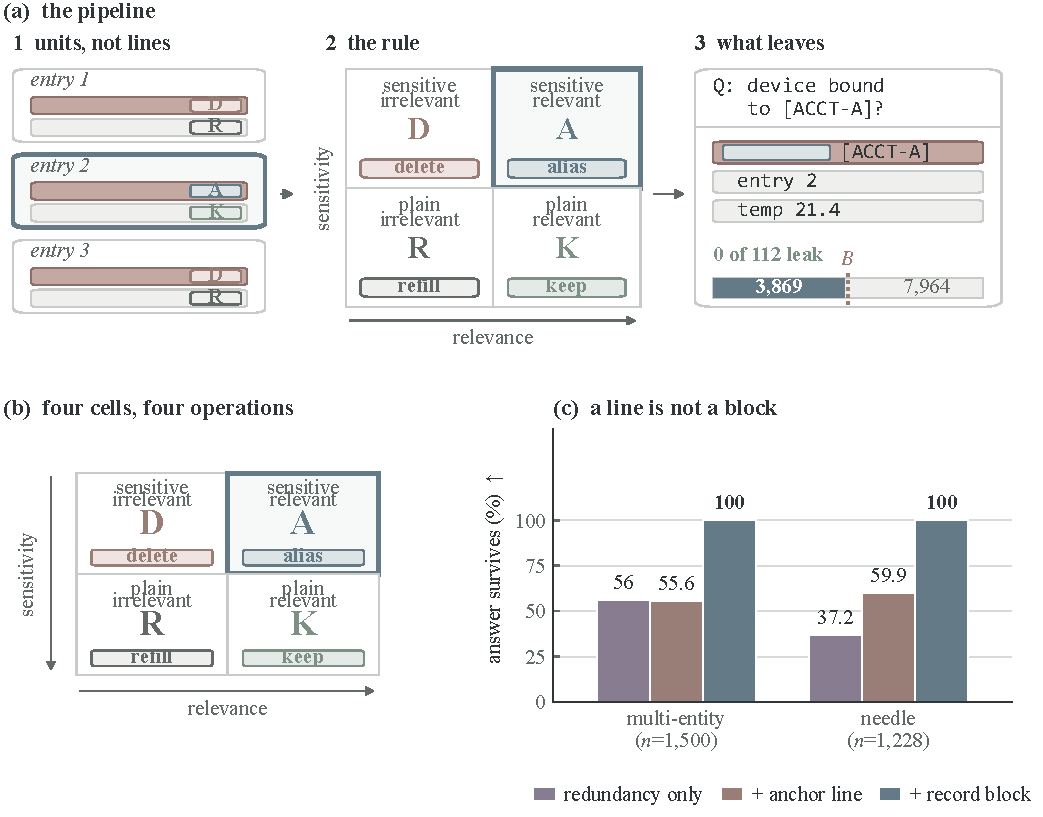
\includegraphics[width=\textwidth]{figures/fig_method.pdf}
\caption{The \textsc{DARK} pipeline. (a) Five stages, all deterministic and model-free.
(1)~An excerpt is split into units inside record blocks, \emph{one line = one unit}.
(2)~Two labels are read off independently: sensitivity from the protected set $V$ that the
operator already holds, relevance from whether the block mentions the entity the question
names---no answer key and no model call enters either.
(3)~The pair selects exactly one operation.
(4)~A keyed map $\kappa$ aliases the protected values and is applied to the question as well;
the entity block is never dropped, and the rest is fitted to $B=\lfloor r\,n_C\rfloor$ in the
stated drop order, with refill units admitted by decreasing redundancy.
(5)~The strip reports a real 112-case run: $3{,}869$ tokens against $7{,}964$, no protected
value in any prompt, F1 $0.6366$.
(b) Why the alias map is keyed. Handing out alias letters in value order makes every alias
invertible from its rank alone; deriving the order from a key removes that signal, and the
question is rewritten through the same map so the two halves still agree.
(c) Protecting the anchor \emph{line} does not close the gap; protecting the \emph{block}
does. Bars give the fraction of the $2{,}728$ cases in which the answer-bearing record
survives.}
\label{fig:pipeline}
\end{figure*}

\begin{algorithm}[t]
\caption{\textsc{DARK} prompt construction}
\label{alg:dark}
\begin{algorithmic}[1]
\Require excerpt $C$, question $q$, budget ratio $r$, protected values $V$
\State $U \gets \textsc{Split}(C)$
\State $A \gets \{u \in U : u \text{ mentions } e^\star(q)\}$
\State $A \gets \textsc{RecordBlock}(U, A)$ \Comment{if $C$ has record markers}
\ForAll{$u \in U$}
  \If{$u \in A$}
     \If{$u$ is sensitive} \State alias($u$) \Comment{sensitive and relevant}
     \Else{} \State keep($u$) \Comment{relevant only}
     \EndIf
  \ElsIf{$u$ is sensitive}
     \State delete($u$) \Comment{sensitive and irrelevant}
  \Else{} \State mark $u$ as refill
  \EndIf
\EndFor
\State $P \gets \textsc{Fit}(\text{kept} \cup \text{aliased}, \text{refill}, B)$
       \Comment{hard $B$; degrade rather than fail}
\State $q' \gets \textsc{AliasQuestion}(q)$ with the same map
\State \Return $(q', P)$
\end{algorithmic}
\end{algorithm}

\subsection{Relevance from the question alone}

The relevance label decides which region must survive and which may be spent on the budget.
We use a single signal: the region containing a mention of the entity the question names.
The signal takes two forms in our excerpts.

\paragraph{Record blocks.}
When the excerpt is segmented into blocks headed by a record marker, the whole block that
contains the anchor mention is relevant. This is the common case for log-shaped benchmarks:
$100\%$ of multi-entity cases and $99.7\%$ of needle cases place the reference answer inside
the same block as the anchor mention. A rule defined on blocks therefore keeps the answer
without inspecting it.

\paragraph{Sentence windows.}
LongBench-style passages carry no block markers. There the relevant region is the anchor
sentence plus one sentence on each side: five units, about $2.3\%$ of the budget in our
measurements. The window is a fallback, not the main mechanism, and
Section~\ref{sec:analysis} reports where it suffices and where it does not.

\paragraph{No answer key.}
A natural implementation of a relevance label is an oracle: mark the unit that contains the
reference answer and deprioritise it last when dropping units. That implementation is not
deployable, and it changes what the method is. We avoid it, and
Section~\ref{sec:analysis} measures how much a pipeline gains from having it, so that the
comparison against an oracle-assisted pipeline is explicit rather than implicit.

\subsection{Four cells, four operations}

Sensitivity is a property of the unit given $V$: a unit is sensitive when it contains a
protected value. Crossing the two labels gives four cells, and each cell receives the
operation that lets the reader resolve the question while the value stays out of the prompt.

\paragraph{Sensitive and relevant: alias (\textbf{A}).}
The unit remains in the context, and each of its protected values is replaced by a stable
alias from a per-run mapping, so that repeated mentions of one entity receive one token.
This cell is where we depart from prior practice. Redaction, the standard primitive, gives
the same concealment but removes the referent. Keeping the unit and renaming its values
preserves the association between the entity and its attributes while satisfying the
constraint on $V$. Section~\ref{sec:analysis} reports the cost of replacing this operation by
deletion: $0.1795$ F1 points overall and $0.3273$ on multi-entity cases.

\paragraph{Sensitive and irrelevant: delete (\textbf{D}).}
The unit holds a protected value that no question component refers to. It contributes
nothing to the answer, so it is removed rather than aliased. This is the only cell in which a
protected value disappears from the prompt entirely.

\paragraph{Relevant and insensitive: keep (\textbf{K}).}
The unit bears on the question and holds nothing that must be hidden, so it is kept verbatim.

\paragraph{Irrelevant and insensitive: refill (\textbf{R}).}
Remaining units hold no protected value and lie outside the relevant region. They compete
for whatever budget is left, ordered by the redundancy score of
Section~\ref{sec:method-budget}.

\subsection{Question-side aliasing}

Aliasing the context alone produces a prompt whose two halves use different names for the
same entity: the context refers to \texttt{[ACCOUNT-A]} while the question still names
\texttt{ACCT-4cd02ed8fb3a}. The reader cannot connect the two, and a string-presence metric
reports the entity as preserved while the task is destroyed. We therefore rewrite the
question with the same map, so that every mention of the queried entity carries the alias
used for it inside the context. The object handed to the model is the pair $(q',P)$, and both
halves are written with one map. Section~\ref{sec:analysis} measures the contribution of
this step.

The alias assignment also determines whether a reader can invert the map by rank. We fix it
per run from a keyed permutation instead of by value order; an unkeyed assignment lets an
adversary who knows the value set recover every alias from its rank alone. All reported
numbers use the keyed assignment.

\subsection{Budget accounting}
\label{sec:method-budget}

The budget is $B=\lceil r\cdot n_C\rceil$, and it is enforced rather than approximated. The
surviving set is assembled greedily and then trimmed against the \emph{actual} concatenated
text, because the separator between units costs tokens: a sum of per-unit token counts is a
lower bound on the length of the joined prompt. When the trimmed set still exceeds $B$,
units are discarded in a fixed priority---refill first, then non-anchor relevant units, then
anchor units---so that the pipeline degrades instead of failing. Every budget arm reported in
this paper has zero overshoot.

Refill ordering uses a model-free redundancy score: for unit $u_i$, the maximum Jaccard
similarity between its token set and that of any other unit. Candidates are visited in
\emph{increasing} redundancy, which keeps the repetitive records.

That direction deserves comment, because it inverts the usual reading of the score. Visiting
units in decreasing redundancy and excluding them is the principled interpretation of a
redundancy measure, and it is what a standard budget-fitting routine does. Here it is the
wrong choice: the answer-bearing record is frequently the most redundant unit, because the
answer value repeats across distractors. Section~\ref{sec:analysis} reports both variants
and the $0.6567$-point difference they produce on the two-hop benchmark. We state the choice
as an empirical regularity with a stated mechanism, not as a consequence of the definition.

\section{Benchmark}
\label{sec:benchmark}

\paragraph{Construction.}
We build the benchmark from six public IoT and smart-home corpora that appear in the
retrieval and long-context literature. For each source we assemble excerpts in which
records for several entities of the same type are interleaved, and we inject synthetic
protected values (account identifiers, contact addresses, phone numbers) into the records
that already exist, rather than into separate carriers. Reference answers are derived
deterministically from the injected structure, so no answer is authored by hand.

The injected values are canaries, not real personal data: public corpora cannot carry real
PII, and using a canary makes leakage measurable exactly. The consequence is that our
privacy claim concerns the recoverability of \emph{these} values, not of arbitrary
personal information that may co-occur in real logs.

\paragraph{Question form.}
Each case poses an entity-resolving question: the question names an account and asks for an
attribute recorded for it (which device is associated, which persona identifier is stored,
and so on). Two families of excerpts are included. In \emph{multi-entity} excerpts the same
question template applies to six accounts and the target account is distinguished only by
its identifier. In \emph{needle} excerpts the question names a specific record identifier
and asks for a field value inside it.

\paragraph{Sizes.}
We report three sets. The \emph{main} set contains $112$ cases, $20$ from each of five
sources and $12$ from a sixth, and is used for the main table, the budget curve, the
cross-model and the paraphrasing experiments. The \emph{extension} set contains $2{,}728$
cases from the same six sources and is used to check that the main-set conclusions survive
an order-of-magnitude increase in size and a different source mix. Both sets share the same
question templates.

A note on key hygiene: the two sets reuse the same case identifiers for different content,
and joining results across them by identifier silently mixes records. Every analysis
reported here (i) resolves results within a single set, and (ii) verifies the join by
comparing the uncompressed-context arm against a reference value computed from the same set.
The check is reported alongside each table.

\paragraph{Public-benchmark variants.}
To test the rule outside our own construction we derive three variants from LongBench
passages, $300$ cases each, with the same injected canaries. \emph{Topical} leaves the
original questions, which name no entity. \emph{Single-hop} replaces the question with one
that names an account, and places the answer in the same record as the account.
\emph{Two-hop} places the answer six sentences away from the account mention, so that
resolving the question requires following the record structure rather than the local
window. Section~\ref{sec:analysis} reports all three, including the one we do not claim.

\section{Experimental Setup}
\label{sec:setup}

\paragraph{Models and decoding.}
The main reader is Qwen2.5-7B-Instruct~\cite{qwen25}; the cross-model check uses
Mistral-7B-Instruct-v0.3~\cite{mistral7b}. Both run in fp16 with greedy decoding,
$64$ new tokens, maximum context $24{,}576$ tokens and a strict policy that aborts rather
than truncates when a prompt exceeds it. The random seed is fixed at \texttt{20261015}.
Scoring uses the official SQuAD~v2 script, a fixed, model-independent procedure.

\paragraph{Baselines.}
We re-run eight published compressors through their reference implementations:
LLMLingua-2~\cite{llmlingua2}, LongLLMLingua~\cite{longllmlingua}, Selective
Context~\cite{selective_context}, Provence~\cite{provence}, CPC~\cite{cpc},
Quito-X~\cite{quitox}, DAC~\cite{dac}, and the Perception
Compressor~\cite{perception_compressor}. Where a method exposes both a budget-matched and a
native configuration we report both; the budget-matched one is used for the headline
comparison, since published defaults vary in length. We additionally run two
sanitization-oriented baselines, INTACT~\cite{intact} and a masking wrapper around
LLMLingua-2, and our own non-routing arms: \arm{full},
\arm{alias} (alias all protected values, no compression), \arm{delete} (redact all, no
compression), \arm{alias\_budget} and \arm{alias\_budget\_link} (global alias, then
redundancy-based selection without and with anchor protection), and the corresponding
\arm{budget\_cluster} pair on raw text.

\paragraph{What each baseline receives.}
All compressors receive the question and the context and nothing else. We verified in the
runner that the reference answer is never passed to any baseline, and that no baseline
consumes the anchor set. This is the fairness condition for the comparison: the
contribution we claim is precisely the ability to obtain the referential benefit without
the answer key.

\paragraph{Equal-budget comparison.}
Budget arms are anchored at $r=0.5$ for the main comparison and swept over
$r\in\{0.10,0.15,0.25,0.50,0.75\}$ for the budget curve. Published compressors are
evaluated at their own $50\%$ setting, with the token accounting reported in every table so
that a method that realises a different length is visible as such.

\paragraph{Statistics.}
All comparisons between two arms on the same cases are paired. We report the mean paired
difference and a $95\%$ percentile bootstrap interval with $10{,}000$ resamples over cases.
A difference is called significant when the interval excludes zero. We deliberately do not
attach a significance claim to any comparison across the two benchmark sizes, which draw
different cases.

\paragraph{Reproducibility controls.}
Two controls are run in every batch. First, the uncompressed arm is recomputed; it involves
no selection logic, so it must reproduce the reference value, and any deviation indicates
that the run differs in model, precision, or data. Second, every budget arm asserts
non-overshoot at the case level. Runs that fail either control are discarded rather than
reported.

\section{Results}
\label{sec:results}

\begin{table}[t]
\caption{Main comparison on the 112-case benchmark (Qwen2.5-7B-Instruct, $r=0.50$, seed
20261015). All arms of ours are constructed without access to the reference answer.
\emph{tokens} is the mean compressed-context length; \emph{leak} counts cases in which a
protected value is recoverable from question plus context. Arrows give the preferred
direction. $BCL$ $=$ \arm{budget\_cluster\_link}, $ABL$ $=$ \arm{alias\_budget\_link},
$ALB$ $=$ \arm{alias\_budget}, $BC$ $=$ \arm{budget\_cluster}. Controlled comparison is the
first three rows: compressing to $48.6\%$ of the original length costs $0.0109$ against the
no-compression aliasing arm, which is not significant. The uncompressed arm is the reference
value used to verify that a result set belongs to this benchmark.}
\label{tab:main}
\centering\small
\setlength{\tabcolsep}{3pt}
\begin{tabular}{lrrr}
\toprule
Arm & F1 $\uparrow$ & tokens $\downarrow$ & leak $\downarrow$ \\
\midrule
\arm{full}                 & 0.7189 & 7964 & 112/112 \\
\arm{alias}                & 0.6475 & 7824 & 0/112 \\
\textbf{\textsc{DARK}} & \textbf{0.6366} & \textbf{3869} & \textbf{0/112} \\
\arm{delete}               & 0.4916 & 7845 & 0/112 \\
BCL                        & 0.4308 & 3683 & 47/112 \\
ABL                        & 0.4219 & 3638 & 0/112 \\
ALB                        & 0.2232 & --- & 0/112 \\
BC                         & 0.2143 & --- & 8/112 \\
\bottomrule
\end{tabular}
\begin{tablenotes}\footnotesize
\item[] Paired differences against \textsc{DARK}: \arm{alias} $-0.0109$
$[-0.0824,+0.0612]$ (n.s.); \arm{full} $-0.0823$ $[-0.1610,-0.0041]$;
ABL $+0.2147$ $[+0.1224,+0.3085]$.
\end{tablenotes}
\end{table}


\subsection{Compression costs little}

Table~\ref{tab:main} answers the first question: at an equal $50\%$ budget, does the routing
rule preserve the task? Aliasing the whole context without compressing scores $0.6475$;
\textsc{DARK} scores $0.6366$ at $48.6\%$ of the tokens. The paired difference is
$-0.0109$ with a $95\%$ interval of $[-0.0824,+0.0612]$, which does not exclude zero: on
this benchmark, halving the context costs no measurable task quality relative to the
leak-free uncompressed arm. Against not compressing and not sanitizing, the deficit is
$-0.0823$ $[-0.1610,-0.0041]$, which is the price of the privacy constraint rather than of
compression, since the aliasing arm pays it as well ($-0.0714$ against \arm{full}).

The comparison specific to our design is the lower block of the table. Two arms are
leak-free and compress to nearly the same length: \arm{alias\_budget\_link}, which aliases
globally and protects the anchor line, and \textsc{DARK}. The difference is $+0.2147$
$[+0.1224,+0.3085]$. The two do not differ in the privacy operation---both alias---but in
which region survives: one line, or the block containing it.

\begin{table*}[t]
\caption{Comparison on the 2{,}728-case extension (Qwen2.5-7B-Instruct, $r=0.50$). Published
compressors are re-run through their reference implementations on the same cases; arms
suffixed \arm{\_native} use each method's own default length. \emph{Leak} is the fraction of
cases in which a protected value is recoverable from the prompt. \textsc{DARK} and the
masking baseline are the only arms at $0\%$; \textsc{DARK} exceeds that baseline by
$+0.3226$ $[+0.3041,+0.3414]$. Against the strongest compressor, Quito-X, the difference is
$+0.0107$ $[-0.0091,+0.0306]$, i.e.\ not significant, at $0\%$ versus $98.1\%$ leakage.
The uncompressed arm reproduces the reference value $0.6078$ from a separately evaluated
batch to within one case in $2{,}728$.}
\label{tab:external}
\centering\small
\setlength{\tabcolsep}{6pt}
\begin{tabular}{llrr}
\toprule
Method & Family & F1 $\uparrow$ & leak $\downarrow$ \\
\midrule
\arm{full}                     & uncompressed       & 0.6081 & 100.0\% \\
\arm{ext\_full}                & uncompressed (rerun) & 0.6078 & 100.0\% \\
\textbf{\textsc{DARK}}     & ours (routes)      & \textbf{0.4937} & \textbf{0.0\%} \\
Quito-X                        & query-aware        & 0.4831 & 98.1\% \\
Quito-X \arm{\_native}         & query-aware        & 0.4862 & 98.1\% \\
CPC                            & query-aware        & 0.4740 & 92.6\% \\
CPC \arm{\_native}             & query-aware        & 0.4523 & 93.4\% \\
Provence                       & query-aware        & 0.4080 & 90.8\% \\
Provence \arm{\_native}        & query-aware        & 0.4047 & 88.8\% \\
\arm{alias\_budget\_link}      & ours, no answer key, merged cell & 0.3482 & 0.0\% \\
\arm{budget\_cluster\_link}    & raw text, anchor kept & 0.3352 & 55.4\% \\
\arm{quad4\_del}               & ours, delete instead of alias & 0.3142 & 0.0\% \\
LLMLingua-2                    & task-agnostic      & 0.2651 & 100.0\% \\
LLMLingua-2 \arm{\_native}     & task-agnostic      & 0.2433 & 100.0\% \\
\arm{mask\_llmlingua2}         & sanitize + compress & 0.1712 & 0.0\% \\
\arm{mask\_llmlingua2\_native} & sanitize + compress & 0.1663 & 0.0\% \\
\arm{alias\_budget}            & global alias, no anchor & 0.1469 & 0.0\% \\
\arm{budget\_cluster}          & redundancy only    & 0.0981 & 0.5\% \\
\bottomrule
\end{tabular}
\end{table*}


\subsection{At scale, the comparison is a privacy comparison}

Table~\ref{tab:external} reports the $2{,}728$-case extension. \textsc{DARK} scores
$0.4937$, level with the strongest query-aware compressor (Quito-X, $0.4831$; difference
$+0.0107$, interval $[-0.0091,+0.0306]$) and above CPC ($0.4740$) and Provence ($0.4080$).
What separates the arms is leakage. Every published compressor leaves protected values in
the prompt, in $88.8\%$ to $100\%$ of cases, because concealing them is not among its
objectives. \textsc{DARK} leaves none. Among leak-free arms the nearest competitor is a
masking wrapper at $0.1712$, which \textsc{DARK} exceeds by $+0.3226$
$[+0.3041,+0.3414]$.

The reading we take from this table is narrow. A query-aware compressor reaches the same F1
as our rule at the same budget, but only by forwarding the value the question names. When
that value must not be forwarded, the compressor loses the task, as the masking row shows,
and the routing rule does not.

\begin{table}[t]
\caption{Budget curve on the 112-case benchmark. Every row satisfies its budget with zero
overshoot. \textsc{DARK} is the strongest budget arm at all five ratios; its advantage
narrows as the budget grows, and its own score peaks at $r=0.50$ because at $r=0.75$ the
additional refill text is noise. The last row gives the mean realised context length in tokens.}
\label{tab:budget}
\centering\small
\setlength{\tabcolsep}{3pt}
\resizebox{\columnwidth}{!}{%
\begin{tabular}{lrrrrr}
\toprule
Arm & @0.10 & @0.15 & @0.25 & @0.50 & @0.75 \\
\midrule
\textbf{\textsc{DARK}} & \textbf{0.4357} & \textbf{0.4681} & \textbf{0.5116} & \textbf{0.6366} & \textbf{0.6158} \\
\arm{quad4\_del}           & 0.3297 & 0.3788 & 0.3955 & 0.5205 & 0.5086 \\
BCL                        & 0.2304 & 0.2052 & 0.2310 & 0.4308 & 0.5576 \\
ABL                        & 0.2304 & 0.2052 & 0.2488 & 0.4219 & 0.5512 \\
\midrule
realised tokens            & 656 & 1033 & 1913 & 3869 & 5830 \\
\bottomrule
\end{tabular}}
\vspace{2pt}
{\footnotesize Uncompressed reference: F1 $0.7189$ at $7964$ tokens.}
\end{table}


\begin{figure*}[t]
\centering
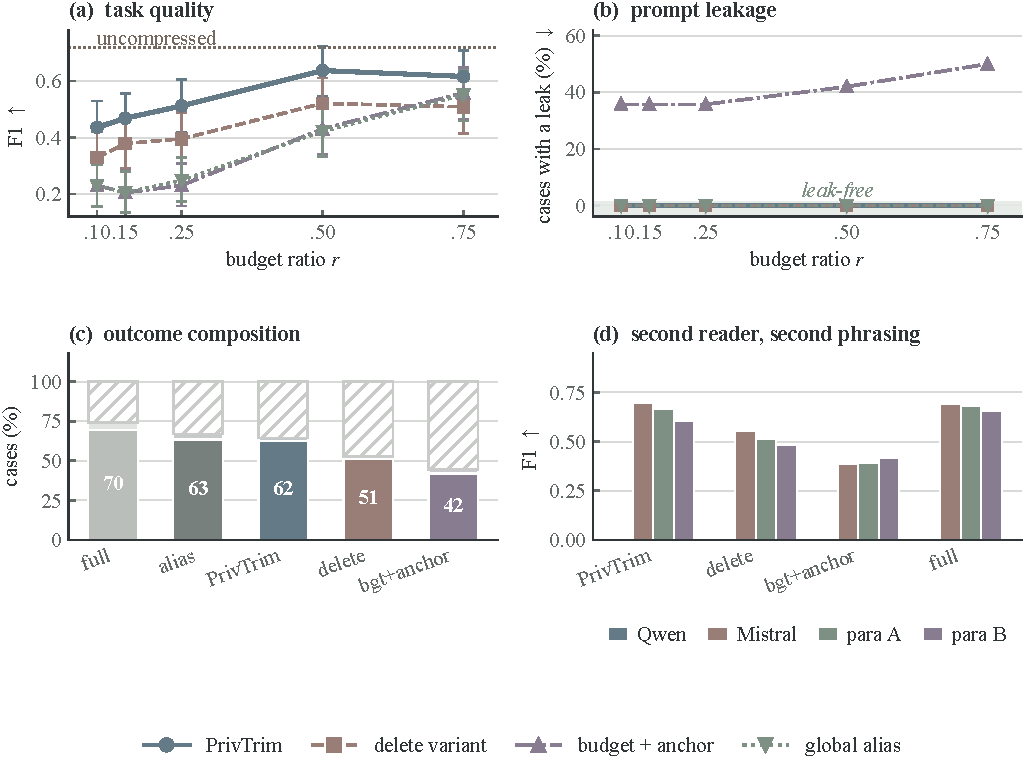
\includegraphics[width=\textwidth]{figures/fig1_main.pdf}
\caption{Behaviour across the budget sweep (112 cases). (a) F1 at five ratios with bootstrap
$95\%$ intervals over cases; the dotted line is the uncompressed reference. (b) Fraction of
cases in which a protected value is recoverable from the prompt. \textsc{DARK}, the
delete variant and the global-alias arm stay at zero for the whole range, while the arm that
compresses raw text leaks in $35.7\%$ of cases at tight budgets and $50.0\%$ at $r=0.75$, so
its apparent parity at loose budgets is bought with exposure. (c) Composition of case
outcomes at $r=0.50$: solid is an exact answer, the pale band is a partial match, hatched is
a wrong or \textsc{unknown} answer. (d) The same four arms under a second reader and two
question paraphrases; the ordering of the arms is preserved in all four conditions.}
\label{fig:budget}
\end{figure*}

\subsection{The advantage holds across budgets}

Table~\ref{tab:budget} varies the budget over five ratios. \textsc{DARK} is the strongest
budget arm at every point: $+0.205$ at $r=0.10$, $+0.263$ at $r=0.25$, $+0.215$ at
$r=0.50$, and $+0.065$ at $r=0.75$, all at zero leakage. Its own score is not monotone. It
peaks at $r=0.50$ and drops by $0.021$ at $r=0.75$, because the additional refill text admitted
at a loose budget is repetitive context that competes with the relevant block for the
reader's attention. The competing arms keep improving with budget, so the margin narrows;
at $r=0.75$ it is small. We report the non-monotonicity rather than describing the curve as
monotone, and note that the half-budget setting used elsewhere is where the mechanism
separates most clearly from the alternatives.

\subsection{Cross-model and phrasing stability}

On Mistral-7B-Instruct-v0.3 at $r=0.50$, \textsc{DARK} scores $0.6946$ against $0.6366$
on Qwen2.5-7B. Every other arm loses ground when the reader changes: \arm{full} $-0.0258$,
\arm{alias} $-0.0544$, \arm{delete} $-0.0357$, \arm{alias\_budget\_link} $-0.0471$,
\arm{budget\_cluster\_link} $-0.0471$. The routing rule is the only arm that improves, which
is consistent with the mechanism: a second reader gains more from a cleaned, budgeted prompt
than from a long one.

Against two mechanical rewritings of the question, \textsc{DARK} scores $0.6637$ and
$0.6023$ against $0.6366$ on the original, a maximum change of $-0.0343$. The uncompressed
arm changes by $-0.0614$ over the same rewritings. The margin over
\arm{alias\_budget\_link} remains significant in all three conditions ($+0.2147$, $+0.2711$,
$+0.1994$). The check is relevant because the rule keys on a mention of the queried entity,
and a rewriting could in principle disturb that mention; in these variants it does not.

\section{Analysis}
\label{sec:analysis}

\begin{table*}[t]
\caption{Isolating the alias-instead-of-delete rule. Replacing the alias operation by
deletion in the sensitive-and-relevant cell, with everything else held fixed, costs a large
and significant amount wherever the anchor is itself a sensitive value (multi-entity,
single-hop, two-hop) and nothing where it is not (topical variants, no anchor). The
two-hop column is the clearest case: the reference answer is present in the context in
$96.3\%$ of cases under the delete variant, and F1 is nevertheless $0.0000$, because the
account that identifies the record has been removed.}
\label{tab:ablation_alias}
\centering\small
\setlength{\tabcolsep}{6pt}
\begin{tabular}{lrrrr}
\toprule
Benchmark & \textsc{DARK} & delete variant & $\Delta$ & 95\% CI \\
\midrule
extension, all ($2{,}728$)     & 0.4937 & 0.3142 & $+0.1795$ & $[+0.1643,+0.1945]$ \\
\quad multi-entity ($1{,}500$) & ---    & ---    & $+0.3273$ & $[+0.3040,+0.3513]$ \\
\quad needle ($1{,}228$)       & ---    & ---    & $-0.0010$ & $[-0.0105,+0.0086]$ (n.s.) \\
main set ($112$)               & 0.6366 & 0.5205 & $+0.1161$ & $[+0.0446,+0.1875]$ \\
LongBench topical ($300$)      & 0.3516 & 0.3503 & $+0.0013$ & $[-0.0002,+0.0042]$ (n.s.) \\
LongBench single-hop ($300$)   & 0.9607 & 0.1674 & $+0.7933$ & $[+0.7430,+0.8426]$ \\
LongBench two-hop ($300$)      & 0.6733 & 0.0000 & $+0.6733$ & $[+0.6200,+0.7256]$ \\
\bottomrule
\end{tabular}
\end{table*}


\subsection{Why redundancy ordering fails here}

The failure we set out to address is not visible in aggregate F1, so we state it in its own
terms. The question is whether the record carrying the answer survives compression when the
rule that decides is a redundancy ordering. On the $2{,}728$-case extension the redundancy-only
rule retains the answer record in $47.5\%$ of cases ($56.0\%$ multi-entity, $37.2\%$ needle),
protecting the anchor line raises this to $57.6\%$, and routing on the record block reaches
$100\%$.

The two failure rates say different things. Multi-entity survival sits either side of the
budget cut, which is what an uninformative ordering produces: the score does not know which
record the question is about, so it keeps the right one about half the time. Needle survival
is \emph{below} the cut, and there the ordering is worse than uninformative. The answer in a
needle case is a field value that recurs across distractor records, so the record holding it
looks like a typical record and inherits no priority from the score. Protecting the anchor
line repairs this for needle cases---retention rises from $37.2\%$ to $59.9\%$---but the line
it protects is not the line that carries the answer, which is why the repair stops short of
$100\%$ rather than reaching it.

Figure~\ref{fig:survival} breaks the same question down by budget, by source, and by what the
retention is worth. Panel (a) follows the answer record across the budget curve: the two arms
that route on the record block hold it in $100\%$ of the 112 cases from $r=0.50$ upward and in
$56.2\%$ at $r=0.10$, while the two arms that only protect the anchor line stay between
$24.1\%$ and $77.7\%$ across the whole range. Panel (b) sets survival against F1 for the
$2{,}728$-case extension. Survival accounts for a good part of the ordering but not all of it:
the delete variant keeps the answer record in $100\%$ of cases and still scores $0.0000$ on
multi-entity cases, because the record it keeps no longer says which account it belongs to. The
dissociation is not an artefact of the aggregate: panel (c) repeats the comparison within each
of the six sources, and the block-level rule holds the answer in every case of every source
while the redundancy-only rule falls to $16.7\%$ on \arm{toolmem\_raw}. Panel (d) shows what
that retention is worth per source; the one source where the block rule is behind, by
$-0.065$, is the one where the redundancy-only arm retains $83.3\%$ and the two are
effectively tied.

\begin{figure*}[t]
\centering
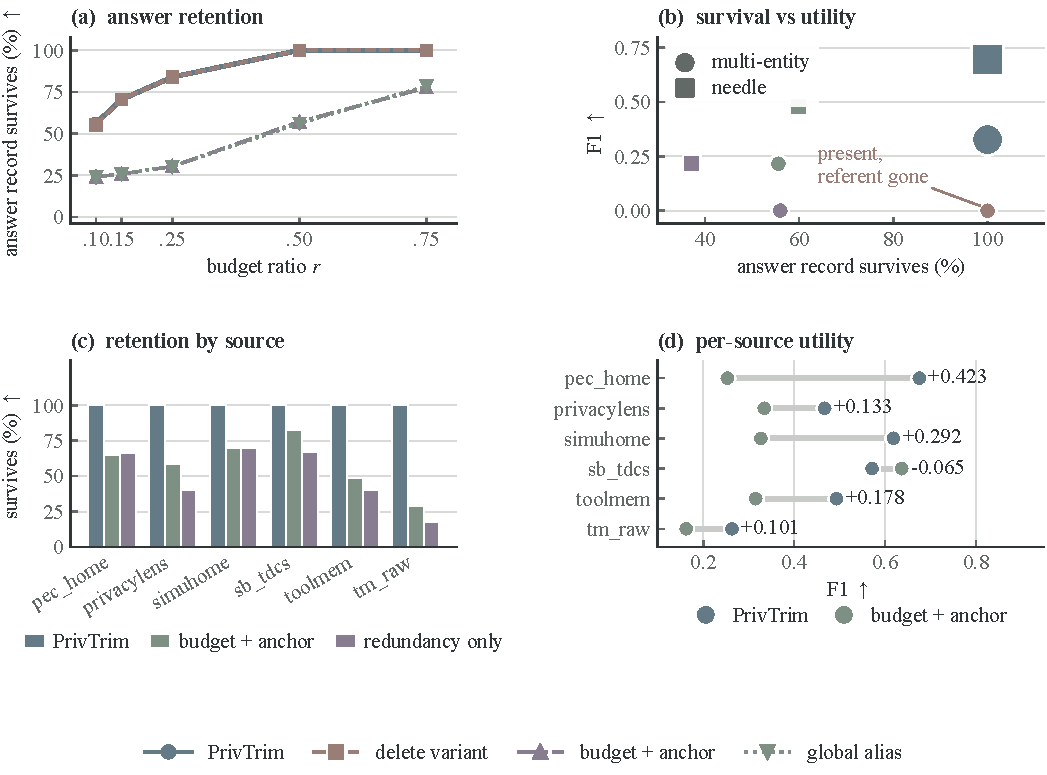
\includegraphics[width=\textwidth]{figures/fig2_diagnostic.pdf}
\caption{Answer retention and what it does not explain. (a) Fraction of the 112 benchmark
cases in which the record carrying the reference answer survives compression, as the budget
varies. \textsc{DARK} and the delete variant coincide almost exactly: the
alias-instead-of-delete rule does not change \emph{which} units survive. (b) Survival against
F1 on the $2{,}728$-case extension; circles are multi-entity cases and squares are needle
cases. The delete variant sits at $100\%$ survival and $0.0000$ F1 on multi-entity cases: the
information is in the prompt and cannot be located. (c) Retention within each source at
$r=0.50$. (d) Per-source F1, \textsc{DARK} against the anchor-protected arm, with the
paired difference printed at each row.}
\label{fig:survival}
\end{figure*}

\subsection{Protecting the anchor line is not enough}

A natural repair forbids dropping units that mention the queried entity. It does not close the
gap, and where it helps it helps for the wrong reason. Overall retention moves from $47.5\%$
to $57.6\%$, but the two families behave differently: multi-entity retention is unchanged
($56.0\%$ to $55.6\%$), while needle retention rises from $37.2\%$ to $59.9\%$. Needle cases
improve because the anchor there is the record identifier, which happens to share the record
with the answer far more often than the account line does. The reason the repair stops short
of $100\%$ is layout: the line carrying the account identifier and the line carrying the
answer are different units in $100\%$ of multi-entity cases and in $65.4\%$ of needle cases.
Preserving the identifier preserves the pointer, not the content.

The repair becomes effective one level up. The excerpt is laid out in record blocks, and the
block containing the anchor mention also contains the answer in $100\%$ of multi-entity cases
and $99.7\%$ of needle cases. Constraining the block instead of the line restores answer
retention to $100\%$ on both families without consulting the answer key. This is the
measurement that motivates the routing rule: the relevant region is a block, not a unit.

\subsection{How much a pipeline gains from the answer key}

Several published pipelines are evaluated with a rule that receives the answer span. Since we
claim to obtain the referential benefit without it, the size of that benefit belongs on the
record. On a 300-case stratified sample, enabling the answer key changes F1 as follows.

\begin{center}\small
\setlength{\tabcolsep}{4pt}
\resizebox{\columnwidth}{!}{%
\begin{tabular}{lcc}
\toprule
Arm & $\Delta$ F1 from answer key $\uparrow$ & 95\% CI \\
\midrule
BC  & $+0.2617$ & $[+0.215,+0.310]$ \\
ALB & $+0.2850$ & $[+0.233,+0.337]$ \\
BCL & $+0.5583$ & $[+0.505,+0.613]$ \\
ABL & $+0.5917$ & $[+0.535,+0.648]$ \\
\bottomrule
\end{tabular}}
\end{center}

The gain is largest for the anchor-protected arms, which are the arms used in the main
comparison. Reporting such a number without the corresponding no-key value would overstate
what a deployed pipeline can do. The tables in Section~\ref{sec:results} report the no-key
values; this entry is here so that the two can be compared.

\subsection{Alias, not delete}

Table~\ref{tab:ablation_alias} and Figure~\ref{fig:aliasdelete} hold everything fixed except
the operation applied in the sensitive-and-relevant cell, and the pattern is the one the
design predicts. Where the anchor is itself a sensitive value, the difference is large and
significant: $+0.3273$ on multi-entity cases, $+0.7933$ on the single-hop variant, $+0.6733$
on the two-hop variant. Where no anchor exists---the topical variant, whose questions name no
entity---it is $+0.0013$ and not significant. On the needle family, whose anchor is a
non-sensitive record identifier, it is $-0.0010$ and not significant.

\begin{figure*}[t]
\centering
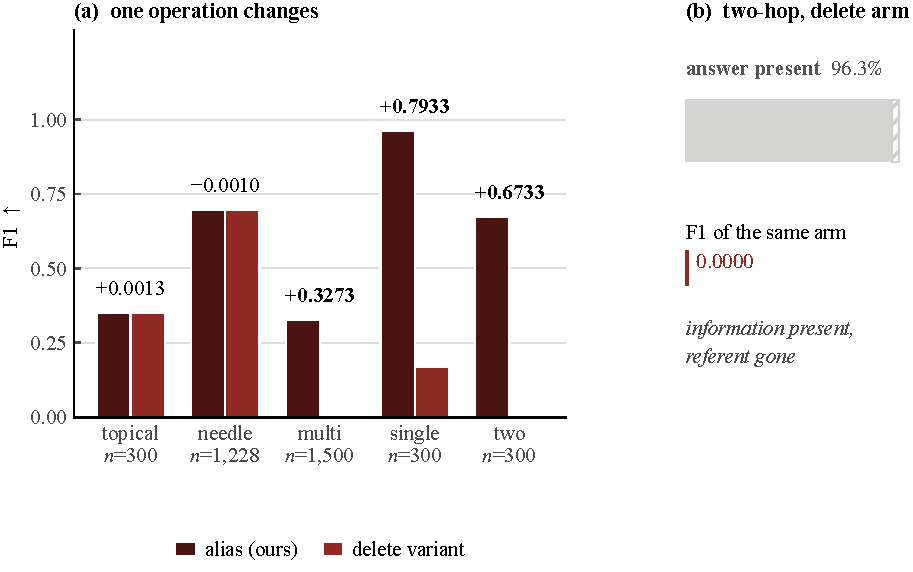
\includegraphics[width=\textwidth]{figures/fig3_alias.pdf}
\caption{Replacing the alias operation by deletion, with the context construction otherwise
unchanged, on five settings. (a) The difference concentrates exactly where the anchor is a
protected value and vanishes where it is not; labels give the paired difference of the two
bars and a star marks an interval that excludes zero. (b) Distribution of the paired per-case
difference for the three settings where the operation matters. The mass sits at both ends
because a case is either answered or not, and the mean gain is largest on the single-hop
variant. (c) In the two-hop variant the answer is still in the prompt after $96.3\%$ of the
deletions, and F1 is zero.}
\label{fig:aliasdelete}
\end{figure*}

% Fig.6 —— 两个真实案例的定性对比（预测为模型实际输出）
\definecolor{anchorbg}{HTML}{DCE4E6}
\definecolor{failbg}{HTML}{F0E4E2}
\definecolor{okbg}{HTML}{E4EAE7}

\begin{figure*}[t]
\centering

\begin{minipage}[t]{0.47\textwidth}
\centering
{\small\bfseries (a) two-hop: the answer sits behind a chain}\\[3pt]
{\scriptsize\itshape Q: which device does account \texttt{ACCT-5f31} operate?}\\[4pt]
\begin{flushleft}\ttfamily\scriptsize\setlength{\parskip}{1.5pt}
\textcolor{black!45}{164}\ \ \colorbox{anchorbg}{\strut account ACCT-5f31} belongs to \colorbox{anchorbg}{\strut user U-5a675c}\\
\textcolor{black!45}{\dots}\\
\textcolor{black!45}{170}\ \ \colorbox{anchorbg}{\strut user U-5a675c} operates device \underline{sensor\_422708\_15}
\end{flushleft}
\vspace{3pt}
{\scriptsize\itshape after aliasing, both links keep a name:}\\[3pt]
\begin{flushleft}\ttfamily\scriptsize
\colorbox{anchorbg}{\strut account [ACCT-A]} belongs to \colorbox{anchorbg}{\strut user [USER-B]}\\
\colorbox{anchorbg}{\strut user [USER-B]} operates device \underline{sensor\_422708\_15}
\end{flushleft}
\end{minipage}\hfill
\begin{minipage}[t]{0.47\textwidth}
\centering
{\small\bfseries (b) multi-entity: the answer looks like a distractor}\\[3pt]
{\scriptsize\itshape Q: which persona id is recorded for account \texttt{ACCT-447f...}?}\\[4pt]
\begin{flushleft}\ttfamily\scriptsize\setlength{\parskip}{1.5pt}
\textcolor{black!45}{07}\ \ \{``device'': ``dehumidifiers'',\\
\phantom{07}\ \ \ ``id'': \underline{``multi\_0166\_00''}, \dots\}\\
\textcolor{black!45}{08}\ \ Private contact record:\\
\textcolor{black!45}{09}\ \ Contact email: contact.e67e...\\
\textcolor{black!45}{11}\ \ \colorbox{anchorbg}{\strut Account ID: ACCT-447fa54ac66d}
\end{flushleft}
\vspace{3pt}
{\scriptsize\itshape the target account is the eleventh of sixteen,}\\
{\scriptsize\itshape and its record is shaped like every other record.}
\end{minipage}

\vspace{7pt}
\resizebox{\textwidth}{!}{%
\begin{tabular}{lcccc}
\toprule
 & \arm{full} & \arm{alias} & \arm{delete} & \textsc{DARK} \\
\midrule
(a)\ \ two-hop, \texttt{lbc-hotpotqa-0000} & \colorbox{okbg}{sensor\_422708\_15} & \colorbox{okbg}{sensor\_422708\_15} & \colorbox{failbg}{UNKNOWN} & \colorbox{okbg}{sensor\_422708\_15} \\
(b)\ \ multi-entity, \texttt{multi-0032} & \colorbox{failbg}{UNKNOWN} & \colorbox{okbg}{multi\_0166\_00} & \colorbox{failbg}{UNKNOWN} & \colorbox{okbg}{multi\_0166\_00} \\
\bottomrule
\end{tabular}}

\caption{Two cases where the routing changes the answer, with the predictions the reader
actually produced. In (a) the question names an account that reaches the answer only through
a user identifier six records later; deleting either link leaves the answer present but
unreachable, and the model returns \textsc{unknown}. In (b) the answer sits in one of sixteen
near-identical account records, so the uncompressed prompt \emph{also} fails---here the
distractor structure, not the budget, is what defeats the reader---while both aliasing arms
answer correctly. Shaded spans mark the names that keep a chain addressable.}
\label{fig:cases}
\end{figure*}


Figure~\ref{fig:cases} shows the two failure modes at the level of a single case, with the
predictions the reader actually produced.

The two-hop column is the most informative single result in this paper. Under the delete
variant the reference answer is present in the context in $96.3\%$ of cases, so GIC is
essentially saturated, and F1 is $0.0000$. The information is in the prompt; the reader
cannot use it, because the identifier saying which record it belongs to has been removed.
String-presence metrics do not detect this failure, which is why we report task quality and
leakage as separate endpoints rather than as one utility score.

\subsection{Question-side aliasing}

Aliasing the context without rewriting the question produces a prompt whose halves use
different names for the same entity. On the 112-case set we measured both settings with the
pipeline otherwise unchanged: \arm{alias} moves from $0.4933$ to $0.6719$ ($+0.1786$) and
\arm{alias\_budget\_link} from $0.5048$ to $0.7450$ ($+0.2402$). The step costs nothing in
privacy, since both halves stay free of the raw value, and it is the difference between a
prompt the reader can use and one it cannot. We therefore treat the pair $(q',P)$ rather
than $P$ alone as the object of study, and verify the mapping before generation.

\subsection{The direction of the refill traversal}

Section~\ref{sec:method-budget} noted that the traversal direction for refill units is an
empirical choice. We ran both variants end to end.

\begin{center}\small
\setlength{\tabcolsep}{4pt}
\resizebox{\columnwidth}{!}{%
\begin{tabular}{lcccc}
\toprule
Benchmark & increasing & decreasing & $\Delta$ & 95\% CI \\
\midrule
extension ($2{,}728$) & 0.4937 & 0.4832 & $-0.0106$ & $[-0.028,+0.007]$ \\
main set ($112$)      & 0.6366 & 0.5844 & $-0.0522$ & $[-0.124,+0.019]$ \\
topical ($300$)       & 0.3516 & 0.3172 & $-0.0344$ & $[-0.090,+0.020]$ \\
single-hop ($300$)    & 0.9607 & 0.9719 & $+0.0111$ & $[-0.008,+0.032]$ \\
two-hop ($300$)       & 0.6733 & 0.0167 & $-0.6567$ & $[-0.712,-0.599]$ \\
\bottomrule
\end{tabular}}
\end{center}

For four of the five rows the interval includes zero. Only the two-hop benchmark separates
the two variants, and it separates them completely. There the answer sits six sentences from
the anchor, outside the fallback window, so whether the answer is present at all is decided
by the refill order; keeping repetitive units happens to retrieve it. We report this as what
it is: an empirical regularity of this data, consistent with the anti-correlation measured at
the start of this section, but not a principled guarantee. The principled remedy is to widen
the relevant region until it covers the answer, which Section~\ref{sec:discussion} takes up.

\subsection{Where the rule applies}

Running the same pipeline on the three LongBench-derived variants locates the boundary.

\begin{center}\small
\setlength{\tabcolsep}{4pt}
\resizebox{\columnwidth}{!}{%
\begin{tabular}{lrrr}
\toprule
Variant & \arm{full} & \arm{alias} & \textsc{DARK} \\
\midrule
topical ($300$)     & 0.4181 & 0.4074 & 0.3516 \\
single-hop ($300$)  & 0.9889 & 0.9197 & 0.9607 \\
two-hop ($300$)     & 0.0967 & 0.7078 & 0.6733 \\
\bottomrule
\end{tabular}}
\end{center}

On the topical variant the questions name no entity, so there is nothing to route on; the
rule degenerates to global aliasing plus redundancy ordering, and it loses $0.0665$ against
the uncompressed prompt. We report that variant as out of scope, not as a success.

The two-hop row carries a second observation we did not anticipate. Without sanitization the
raw prompt scores $0.0967$; with global aliasing it scores $0.7078$. The account identifiers
in this variant are long hexadecimal strings differing in a few characters, and replacing
them with short distinct tokens makes the task \emph{easier} for the reader. Privacy and
utility move in the same direction here, which is a useful counterpoint to the usual framing
but also a reminder that the effect belongs to the identifier surface form, not to the
routing rule.

\section{Discussion}
\label{sec:discussion}

\paragraph{The scope the evidence supports.}
The claim we support is bounded. For excerpts of IoT-style operational records, queried by a
question that names an entity whose value must not reach the model, routing each unit on
(sensitivity, relevance) and aliasing the sensitive-and-relevant cell preserves the task at
half the tokens and at zero measured leakage. The three variants in
Section~\ref{sec:analysis} delimit it: the rule is unnecessary when the question is topical,
redundant when anchor and answer coincide in a single record, and dependent on the refill
order when the answer lies outside the fallback window. We do not claim that it improves
ordinary compression on ordinary prompts, and the topical variant shows that it does not.

\paragraph{What the privacy claim covers.}
Leakage is measured as recoverability of the protected values from the exact prompt text,
using the pattern set of the published protocol (full value plus fragments). That is the
relevant quantity for a pipeline whose adversary is the model provider and whose prompts may
be retained. It is not a formal guarantee. We derive no differential-privacy
bound~\cite{dp} and no $k$-anonymity guarantee~\cite{kanon}; the alias map is assumed private,
and an adversary who obtains it recovers the values. We fix the alias assignment from a keyed
permutation precisely so that an adversary holding only the value set cannot invert the map
by rank, which is a real attack on unkeyed assignment, but that mitigation is narrower than a
guarantee. We also do not evaluate inference attacks---membership, attribute, or the
reconstruction of a value from its alias's co-occurrence pattern---and none of them is
addressed by the present evidence.

\paragraph{The refill order is a regularity.}
The measured benefit of keeping repetitive units follows from an anti-correlation between
redundancy and answer-bearing in this data. It is not derived from the definition of the
score, and a corpus whose answers are unique rather than repeated would not exhibit it. The
principled fix is to make the relevant region cover the answer instead of relying on the
ordering. In the two-hop variant the answer lies at a fixed distance of six sentences from
the anchor, so a window of that width would protect it explicitly and remove the dependence.
We have not run that configuration, and the present results should be read as depending on
the fallback width.

\paragraph{Cost.}
Prompt construction is lexical and model-free: one pass over the units to label them, one
pass to score redundancy (quadratic in the number of units in the worst case), and one pass
to fit the budget. It adds no model call. On the longest excerpt in the extension set
($19{,}838$ tokens uncompressed) construction completes in under a second on CPU. We did not
measure end-to-end wall-clock or memory of the reader, so the efficiency we claim concerns
prompt length rather than latency.

\paragraph{Threats to validity.}
The protected values are synthetic canaries injected into public corpora, because those
corpora cannot carry real personal data. Canary leakage is measurable exactly, but the
measured rate is a property of this construction. Both benchmark sizes are generated by our
own scripts from shared templates, so the questions are entity-resolving by construction and
the two-hop distance is fixed rather than sampled. The readers are 7B-parameter
instruction-tuned models, and we have no evidence about larger or API-served models. Finally,
the two benchmark sizes reuse case identifiers for different content, so a cross-set join by
identifier would silently mix records; we guard against this by verifying the uncompressed
arm against a per-set reference value, but the hazard is worth stating for anyone reusing the
artifacts.

\section{Conclusion}
\label{sec:conclusion}

We studied what happens to a privacy-preserving inference pipeline when the entity a
question asks about is also the entity that must be protected. Two standard remedies fail
there, for opposite reasons. Redaction removes the referent the reader needs. Redundancy
ordering removes the record that carries the answer, because on this data the answer-bearing
record is the most repetitive one. We presented \textsc{DARK}, which resolves the conflict
by deciding the two axes per unit and by giving the sensitive-and-relevant cell an operation
that neither remedy provides: the unit stays, its values are aliased, and the same map is
applied to the question. Relevance is read off the question---the record block that mentions
the queried entity---so the pipeline needs neither a reference answer nor training.

Across a 112-case benchmark over six public datasets, \textsc{DARK} uses $48.6\%$ of the
tokens at zero prompt-level leakage and is statistically indistinguishable from aliasing the
full context without compression ($-0.0109$). On a $2{,}728$-case extension it matches the
strongest query-aware compressor ($+0.0107$, not significant) at $0\%$ leakage against
$98.1\%$, and exceeds the nearest leak-free baseline by $0.3226$ F1 points. A single
controlled substitution isolates the decision behind these numbers: replacing the alias
operation with deletion costs $0.1795$ F1 points overall, $0.3273$ on multi-entity cases, and
nothing where no anchor exists. The last figure matters as much as the others, because it
indicates that the rule acts on the structure it was designed for and is inert elsewhere.

Two directions follow from the limits stated in Section~\ref{sec:discussion}. The fallback
window is the weakest part of the mechanism: in the two-hop variant the answer lies outside
it and is recovered only through the refill order, so widening the relevant region to cover
the answer is the first configuration to test. The second concerns the privacy claim itself.
A pipeline of this shape would be considerably stronger with a guarantee that survives an
adversary holding the alias map, and establishing one is a different piece of work from the
one reported here.


\balance
\bibliographystyle{plainnat}
\bibliography{refs}

\appendix
\section{Appendix}
\label{sec:appendix}

\subsection{Per-source breakdown}

\paragraph{Extension set ($2{,}728$ cases).}
F1 by source, budget $r=0.50$, all arms of ours constructed without the answer key. The
routing rule is strongest on \arm{pec\_home} and \arm{smartbench\_tdcs} and weakest on
\arm{toolmem\_raw}, where the uncompressed arm is also weakest.

\begin{table}[t]
\caption{Per-source F1 on the extension set ($2{,}728$ cases, $r=0.50$).}
\label{tab:app_persource_ext}
\centering\small
\setlength{\tabcolsep}{3pt}
\resizebox{\columnwidth}{!}{%
\begin{tabular}{lrrrr}
\toprule
Source & $n$ & \arm{full} & \textsc{DARK} & ABL \\
\midrule
\arm{pec\_home}        & 426 & 0.7816 & 0.6756 & 0.2859 \\
\arm{privacylens}      & 600 & 0.5340 & 0.4671 & 0.3381 \\
\arm{simuhome}         & 312 & 0.8686 & 0.6186 & 0.3910 \\
\arm{smartbench\_tdcs} & 490 & 0.6449 & 0.5714 & 0.6367 \\
\arm{toolmem}          & 300 & 0.5154 & 0.4933 & 0.3121 \\
\arm{toolmem\_raw}     & 600 & 0.4401 & 0.2631 & 0.1624 \\
\midrule
overall                & 2728 & 0.6081 & 0.4937 & 0.3482 \\
\bottomrule
\end{tabular}}
\end{table}

\paragraph{Main set ($112$ cases).}
Same setting on the smaller set.

\begin{table}[t]
\caption{Per-source F1 on the main set ($112$ cases, $r=0.50$).}
\label{tab:app_persource_main}
\centering\small
\setlength{\tabcolsep}{3pt}
\resizebox{\columnwidth}{!}{%
\begin{tabular}{lrrrr}
\toprule
Source & $n$ & \arm{full} & \textsc{DARK} & \arm{alias} \\
\midrule
\arm{pec\_home}        & 20 & 0.8750 & 0.8250 & 0.8250 \\
\arm{privacylens}      & 20 & 0.6567 & 0.6400 & 0.4900 \\
\arm{simuhome}         & 20 & 0.8500 & 0.7500 & 0.7500 \\
\arm{smartbench\_tdcs} & 20 & 0.7000 & 0.7000 & 0.6500 \\
\arm{toolmem}          & 12 & 0.4901 & 0.4167 & 0.4354 \\
\arm{toolmem\_raw}     & 20 & 0.6500 & 0.4000 & 0.6500 \\
\midrule
overall                & 112 & 0.7189 & 0.6366 & 0.6475 \\
\bottomrule
\end{tabular}}
\end{table}

\subsection{Anchor types covered}

The anchor key is resolved differently depending on what the question names. All six forms
occurring in the extension set are handled, and the anchor string is present in the context
in every case ($2{,}728/2{,}728$).

\begin{table}[htbp]
\caption{Anchor key forms covered by the routing rule. All six occur in the extension set and
the anchor string is present in the context in every case ($2{,}728/2{,}728$).}
\label{tab:app_anchor}
\centering\small
\setlength{\tabcolsep}{3pt}
\resizebox{\columnwidth}{!}{%
\begin{tabular}{llr}
\toprule
\arm{anchor\_kind} & Example question form & $n$ \\
\midrule
none (entity field) & \emph{for account} \texttt{ACCT-\ldots} & 1500 \\
\arm{id}            & \emph{for record id} \texttt{pec\_home\_\ldots} & 316 \\
\arm{name}          & names an entity directly & 300 \\
\arm{session}       & names a session & 300 \\
\arm{entry}         & \emph{for entry 3} & 281 \\
\arm{native}        & native identifier & 31 \\
\bottomrule
\end{tabular}}
\end{table}

\subsection{Leakage counting}

A case counts as leaking when any protected value, or a fragment of it, is recoverable from
the concatenation of the rewritten question and the compressed context. Fragments are the
pattern set of the published protocol. The count is per case, not per value, so the reported
rate is the fraction of cases with at least one exposure; the per-value count is retained in
the artifacts.

\subsection{Reproduction notes}

Every table in this paper is computed from per-case records that ship with the artifacts, one
line per (case, arm). The uncompressed arm in each set is used as an identity check: a result
set whose uncompressed arm does not reproduce the reference value is not part of this paper.
Budget arms assert non-overshoot per case; a run that violates it is discarded rather than
truncated. All arms of ours are keyed alias runs; an unkeyed assignment changes both the
alias strings and the resulting score, so results are only comparable within one setting.


\end{document}
